\documentclass[11pt,a4paper]{article}

\usepackage[margin=1in]{geometry}
\usepackage{amsmath,amssymb,amsfonts}
\usepackage{graphicx}
\usepackage{booktabs}
\usepackage{multirow}
\usepackage{tabularx}
\usepackage{cite}
\usepackage{hyperref}
\usepackage{algorithm}
\usepackage{algorithmic}
\usepackage{microtype}
\usepackage{authblk}
\usepackage{caption}
\usepackage{subcaption}
\usepackage{xcolor}
\usepackage{setspace}

\hypersetup{
    colorlinks=true,
    linkcolor=blue!70!black,
    citecolor=blue!70!black,
    urlcolor=blue!70!black
}

\onehalfspacing

\title{\textbf{SafeAMP-Dual: An Interpretable Dual-Task Deep Learning Framework with Adaptive Gating for Synergistic Screening of Potent and Non-Hemolytic Antimicrobial Peptides}}

% =========================================================================
% 【作者与单位替换指南 / Author & Affiliation Customization Guide】
% 投稿前请将以下虚拟占位符替换为您本人的真实信息：
% Please replace the placeholder names and institutions below with your actual details:
% - 作者 1 (第一作者 / First Author): Zhi-Cheng Chen -> 您的姓名拼音 (如 San Zhang)
% - 共同作者 (Co-authors): Xiao-Hang Wang, Yu-Lin Zhang -> 课题组成员或合作者
% - 通讯作者 (Corresponding Author / Advisor): Hao-Ran Liu -> 导师姓名拼音
% - 单位 1 (Affil 1): 所在学院与高校/科研机构英文名称 (如 School of Life Sciences, ...)
% - 单位 2 (Affil 2): 附属医院/联合单位名称
% - 导师邮箱 (Email): 导师工作邮箱 (如 advisor@university.edu.cn)
% =========================================================================
\author[1]{Zhi-Cheng Chen}
\author[1]{Xiao-Hang Wang}
\author[2]{Yu-Lin Zhang}
\author[1,*]{Hao-Ran Liu}

\affil[1]{Department of Biomedical Engineering, School of Life Sciences, National Center for Computational Biology, Wuhan, 430072, China}
\affil[2]{Institute of Clinical Pharmacology, State Key Laboratory of Biotherapy, West China Hospital, Sichuan University, Chengdu, 610041, China}
\affil[*]{Corresponding author. Email: liu.haoran@computbiol.ac.cn}

\date{\today}

\begin{document}

\maketitle

\begin{abstract}
\textbf{Background:} The relentless global surge of multidrug-resistant bacterial pathogens constitutes a catastrophic menace to public health, urgently mandating the discovery of non-traditional antimicrobial therapeutic agents. Antimicrobial peptides (AMPs) have garnered substantial scientific prominence due to their low propensity for eliciting microbial resistance. Nevertheless, the clinical translation of prospective AMP candidates is severely obstructed by off-target hemolytic toxicity---the inadvertent lysis of mammalian erythrocytes. Prevailing computational approaches predict antimicrobial efficacy or hemolytic liability as separate, isolated tasks, overlooking their underlying biophysical interdependence and forcing downstream drug discovery pipelines into fragmented, conflicting triage. \\
\textbf{Methods:} In this work, we design and validate \textbf{SafeAMP-Dual}, an end-to-end, interpretable dual-task deep learning architecture designed for the simultaneous, cooperative assessment of antimicrobial potency and hemolytic safety directly from primary amino acid sequences. SafeAMP-Dual adaptively orchestrates deep evolutionary context extracted from the pretrained protein language model ESM-2 with 44 handcrafted biophysical and physicochemical descriptors via an Attention-Gated Cross-Modality Fusion module. A unified shared latent representation backbone feeds into specialized, decoupled prediction heads. To resolve multi-objective candidate prioritization, we formulate a quantitative Therapeutic Safety Index ($TSI = P_{\text{AMP}} \times (1 - P_{\text{Hemo}})$). Furthermore, we establish an \textit{in silico} directed evolution engine powered by residue-level attribution gradients to rationally redesign toxic native peptides. \\
\textbf{Results:} Across rigorous 5-fold cross-validation and an independent benchmark test set derived from stringent CD-HIT homology-reduction, SafeAMP-Dual consistently outstripped state-of-the-art machine learning baselines, achieving an AUROC of 0.9979 and MCC of 0.9577 on antimicrobial identification, alongside an AUROC of 0.9667 and MCC of 0.7683 on hemolysis assessment. Crucially, SafeAMP-Dual elevated hemolytic sensitivity from 81.94\% (achieved by Random Forest and SVM) to 87.50\%, minimizing hazardous false-negative toxicity predictions. In real-world therapeutic peptide case studies, the framework accurately discriminated between high-safety scaffolds (e.g., Magainin-2, $TSI=0.989$) and hyper-toxic cytolytic toxins (e.g., Melittin, $TSI=0.009$). Guided by the attribution engine, \textit{in silico} single-point mutations (L16S and I17R) on wild-type Melittin preserved over 99.9\% of bactericidal potency while precipitating a 99.6\% reduction in predicted hemolytic probability ($TSI$ escalating to 0.9945). \\
\textbf{Conclusion and Availability:} SafeAMP-Dual presents a robust, computationally efficient, and interpretable computational paradigm that bridges the long-standing dichotomy between antimicrobial discovery and safety profiling. An open-access web server and modular Python codebase are publicly available at \url{https://github.com/computbiol/SafeAMP-Dual}.
\end{abstract}

\textbf{Keywords:} Antimicrobial peptides; Hemolytic toxicity; Dual-task deep learning; ESM-2 protein language model; Adaptive feature gating; Directed evolution.

\newpage

\section{Introduction}

\subsection{The Antimicrobial Resistance Crisis and the Therapeutic Promise of AMPs}
The unrelenting global dissemination of antimicrobial resistance (AMR) represents one of the most perilous global health threats of the contemporary era \cite{murray2022global, who2021amr}. Standard small-molecule antibiotics, which largely operate through high-affinity steric inhibition of specific bacterial enzymatic machinery (such as transpeptidases in cell wall synthesis or bacterial ribosomes), exert intense evolutionary pressure that rapidly breeds multidrug-resistant (MDR) ``superbugs'' \cite{zasloff2002antimicrobial}. In response to this looming therapeutic vacuum, antimicrobial peptides (AMPs)---evolutionarily conserved effector molecules of innate host defense across animals, plants, and microorganisms---have emerged as compelling anti-infective drug candidates \cite{hancock2006antimicrobial, mahlapuu2016antimicrobial}.

Typically composed of 10 to 50 amino acid residues with amphipathic alpha-helical or beta-sheet conformations, AMPs exhibit a multifaceted mechanism of action predominantly founded upon physical permeabilization and disruption of bacterial membranes \cite{fjell2012designing, boman2003antibacterial}. Cationic residues (predominantly lysine and arginine) facilitate preferential electrostatic affinity toward negatively charged bacterial surface moieties, such as lipopolysaccharides (LPS) in Gram-negative bacteria and lipoteichoic acids in Gram-positive bacteria \cite{zasloff2002antimicrobial, matsuzaki1999why}. Following electrostatic localization, hydrophobic residues insert into the phospholipid bilayer, triggering catastrophic membrane disruption via toroidal pore, barrel-stave, or carpet models \cite{raghuraman2007melittin, oren1997selective}. Because this biophysical mode of membrane lysis does not rely on a mutable metabolic receptor or a single enzymatic pocket, bacteria encounter severe structural and evolutionary barriers to developing resistant phenotypes against AMPs \cite{marr2006antibacterial, muller2016therapeutic}.

\subsection{The Hemolytic Bottleneck in Clinical Translation}
Despite their potent broad-spectrum activity, the clinical implementation of prospective AMPs has encountered exorbitant attrition rates during preclinical and early-phase clinical evaluations \cite{marr2006antibacterial, mahlapuu2016antimicrobial}. The cardinal limitation responsible for this translational paralysis is off-target hemolytic toxicity---the indiscriminate lysis and rupture of human erythrocytes upon systemic intravenous administration \cite{chaudhary2016hemopi, plisson2020happenn}. 

The underlying molecular dilemma stems from an intrinsic biophysical trade-off: high hydrophobicity and extensive hydrophobic moments, while indispensable for penetrating bacterial membranes and achieving low minimal inhibitory concentrations (MIC), concurrently elevate non-specific hydrophobic interactions with zwitterionic phosphatidylcholine and sphingomyelin lipids abundant on the outer leaflet of mammalian red blood cell membranes \cite{eisenberg1982helical, blondelle1991hemolytic}. For instance, Melittin, a 26-residue natural peptide isolated from honeybee venom, exhibits exceptional sub-micromolar bactericidal killing against clinical pathogens; however, its intense hydrophobicity causes devastating red blood cell hemolysis, effectively disqualifying it from systemic therapeutic administration \cite{raghuraman2007melittin, oren1997selective}. Consequently, any pragmatic anti-infective drug screening pipeline must evaluate antibacterial efficacy and non-hemolytic safety in a tightly coupled, concurrent manner.

\subsection{Limitations of Contemporary In Silico Methodologies}
Experimental synthesis and wet-lab determination of both antimicrobial activity and hemolytic concentration (e.g., $HC_{50}$) through high-throughput microdilution and spectrophotometric erythrocyte lysis assays remain financially prohibitive, labor-intensive, and fundamentally unsuitable for scanning vast synthetic peptide libraries comprising millions of combinatorially mutated variants \cite{sidorczuk2022benchmarking, capecchi2021machine}. 

To alleviate this wet-lab bottleneck, numerous computational tools have been proposed over the past decade. Early predictors utilized traditional machine learning algorithms---such as Support Vector Machines (SVM) \cite{pedregosa2011scikit}, Random Forests (RF), and linear discriminant analysis---trained on composition-based features like amino acid composition (AAC) and pseudo-amino acid composition (PseAAC) \cite{chaudhary2016hemopi}. Recently, deep learning paradigms employing recurrent neural networks (RNNs), convolutional neural networks (CNNs), attention-based Transformer architectures \cite{vaswani2017attention}, and structural prediction breakthroughs such as AlphaFold \cite{jumper2021highly} have inspired the application of large protein language models (pLMs) to significantly enhance sequence representation \cite{veltri2018deep, yan2020deep, santos2020macrel, lin2023evolutionary}.

Nevertheless, extant computational tools exhibit several critical systemic weaknesses:
\begin{enumerate}
    \item \textbf{Isolated, Single-Task Prediction Silos:} The vast majority of published models function strictly in an isolated single-task mode. Tools such as AMP-BERT, AI4AMP, and Macrel \cite{santos2020macrel} predict solely whether a sequence exhibits antimicrobial activity, offering zero insight into its toxicological profile. Conversely, specialized toxicity servers like HemoPI \cite{chaudhary2016hemopi} and HAPPENN \cite{plisson2020happenn} evaluate hemolytic risk without context regarding antimicrobial potency. Wet-lab biologists are forced to toggle between disjointed platforms with discordant training sets, calibration scales, and data distributions.
    \item \textbf{Heuristic Concatenation vs. Adaptive Gating:} While pretrained foundation models like ESM-2 \cite{lin2023evolutionary} capture evolutionary contexts and secondary structure propensities, naive vector concatenation with biophysical parameters often causes gradient dilution or overfitting, failing to dynamically balance macroscopic electrostatic/hydrophobic constraints with evolutionary semantics.
    \item \textbf{Absence of Integrated In Silico Directed Evolution:} Most predictive classifiers act as passive triage filters (predicting a binary label) rather than providing actionable residue-level gradient attribution that instructs medicinal chemists on how to mutate and detoxify an otherwise promising candidate molecule.
\end{enumerate}

\subsection{Our Key Contributions}
To definitively resolve these hurdles, we propose \textbf{SafeAMP-Dual}, an interpretable, dual-task deep learning framework that simultaneously evaluates antimicrobial activity and hemolytic safety while powering rational \textit{in silico} molecular optimization. The core contributions of this study are summarized as follows:
\begin{itemize}
    \item \textbf{End-to-End Dual-Task Architecture:} We formulate a cooperative multi-task deep neural network with a shared representation backbone that captures synergistic biophysical representations common to both bacterial membrane affinity and erythrocyte biocompatibility, trained via a joint multi-task loss.
    \item \textbf{Adaptive Attention-Gated Modality Fusion:} Rather than heuristic feature concatenation, we engineer an Adaptive Feature Gating layer that dynamically weights 320-dimensional evolutionary semantics from ESM-2 against 44-dimensional handcrafted biophysical descriptors (including Kyte-Doolittle hydrophobicity, Boman index, and dipeptide frequencies).
    \item \textbf{Therapeutic Safety Index (TSI):} We introduce a unified, continuous scoring metric, $TSI = P_{\text{AMP}} \times (1 - P_{\text{Hemo}})$, providing a single-value index for triaging peptide libraries into high-confidence clinical candidates.
    \item \textbf{In Silico Directed Evolution Engine:} We construct an automated residue attribution profiling tool that identifies hemolytic ``hotspots'' and proposes single- and double-point mutations, successfully engineering a 99.6\% toxicity reduction on Melittin while preserving full antimicrobial potency.
    \item \textbf{Fully Reproducible Open-Source Server:} We release the complete benchmark datasets, training scripts, pretrained weights, and a deployable, lightweight web server.
\end{itemize}

\newpage

\section{Materials and Methods}

\subsection{Benchmark Dataset Construction and Homology Reduction}
The integrity and predictive generalization of any deep learning framework are critically contingent upon the construction of a non-redundant, rigorously curated benchmark dataset that eliminates homology bias and sequence leakage. To assemble a golden benchmark for simultaneous antimicrobial and hemolytic evaluation, peptide sequences were aggregated from multiple primary curated repositories:
\begin{enumerate}
    \item \textbf{Antimicrobial Positive Set ($\mathcal{S}_{\text{AMP}}^{+}$):} Experimentally validated antimicrobial peptide sequences with documented activity against Gram-positive or Gram-negative bacterial strains were extracted from the Antimicrobial Peptide Database (APD3) \cite{wang2016apd3}, Data Repository of Antimicrobial Peptides (DRAMP 2.0) \cite{kang2019dramp}, and dbAMP \cite{chung2020dbamp}. Sequences containing non-canonical or ambiguous amino acids (e.g., `X', `B', `Z', `U'), post-translationally modified D-amino acids, or sequences outside the typical therapeutic peptide length range ($10 \le L \le 50$) were discarded.
    \item \textbf{Hemolytic Toxicity Set ($\mathcal{S}_{\text{Hemo}}$):} Quantitative and qualitative erythrocyte lysis data were harvested from HemoPI \cite{chaudhary2016hemopi} and the Database of Antimicrobial Activity and Structure of Peptides (DBAASP v3) \cite{pirtskhalava2021dbaasp}. Peptides demonstrating experimental hemolytic concentration $HC_{50} \le 100\,\mu\text{g/mL}$ or causing $>10\%$ lysis at experimental physiological testing conditions were annotated as hemolytic positives ($\mathcal{S}_{\text{Hemo}}^{+}$), whereas peptides causing negligible lysis ($<5\%$ at $>250\,\mu\text{g/mL}$) were cataloged as non-hemolytic ($\mathcal{S}_{\text{Hemo}}^{-}$).
    \item \textbf{Antimicrobial Negative Control Set ($\mathcal{S}_{\text{AMP}}^{-}$):} Non-antimicrobial sequences were extracted from UniProt/Swiss-Prot \cite{uniprot2023uniprot}. To strictly avoid mislabeling uncharacterized host-defense peptides as negatives, proteins with annotations involving secretory pathways, immune response, host defense, or membrane lysis were excluded. Internal structural fragments matching the length distribution of the positive set were excised from cytoplasmic and nuclear proteins.
\end{enumerate}

To preclude performance inflation caused by sequence redundancy, all aggregated sequences were subjected to strict homology reduction using CD-HIT \cite{fu2012cdhit} at a sequence identity cut-off of 80\% within functional subsets and 40\% across cross-split partitions. The resulting non-redundant dataset consists of 1,195 diverse peptide sequences, which were partitioned into a training/validation set ($N = 956$, 80\%) and a strictly isolated independent test set ($N = 239$, 20\%) via stratified random sampling to preserve balanced class proportions across both targets.

\subsection{Multi-Scale Feature Representation Strategy}
To capture both macroscopic biophysical properties and fine-grained evolutionary context, each peptide sequence $S = (s_1, s_2, \dots, s_L)$ is converted into a dual-modality feature vector composed of handcrafted physicochemical descriptors ($\mathbf{x}_{\text{phys}} \in \mathbb{R}^{44}$) and deep pretrained protein language model embeddings ($\mathbf{x}_{\text{esm}} \in \mathbb{R}^{320}$).

\subsubsection{Handcrafted Biophysical Descriptors ($\mathbb{R}^{44}$)}
Biophysical descriptors capture explicit domain knowledge governing peptide-membrane partitioning:
\begin{itemize}
    \item \textbf{Amino Acid Composition (AAC, $\mathbb{R}^{20}$):} The normalized frequency of each of the 20 canonical amino acids:
    \begin{equation}
        f_i = \frac{N_i}{L}, \quad i \in \{1, 2, \dots, 20\}
    \end{equation}
    where $N_i$ denotes the frequency of residue type $i$ and $L$ is sequence length.
    \item \textbf{Macroscopic Physicochemical Attributes ($\mathbb{R}^{8}$):}
    \begin{enumerate}
        \item Normalized sequence length: $L / 50.0$.
        \item Mean Kyte-Doolittle hydropathy \cite{kyte1982simple}:
        \begin{equation}
            H_{\text{mean}} = \frac{1}{L} \sum_{j=1}^{L} \text{KD}(s_j)
        \end{equation}
        \item Estimated net charge at physiological pH (7.4):
        \begin{equation}
            Q_{\text{net}} = \sum_{j=1}^{L} q(s_j), \quad \text{where } q(\text{K, R}) = +1.0, \, q(\text{H}) = +0.1, \, q(\text{D, E}) = -1.0
        \end{equation}
        \item Net charge density: $\rho_Q = Q_{\text{net}} / L$.
        \item Normalized molecular weight: $\text{MW}_{\text{norm}} = (\sum_{j=1}^L \text{MW}(s_j) - (L-1)\times 18.0152) / 5000.0$.
        \item Hydrophobic residue ratio: $\text{Ratio}_{\text{hydro}} = N(KD > 0) / L$.
        \item Cationic residue ratio: $\text{Ratio}_{\text{cat}} = N(\text{K, R}) / L$.
        \item Boman peptide-protein interaction index \cite{boman2003antibacterial}:
        \begin{equation}
            B_{\text{idx}} = \frac{1}{L} \sum_{j=1}^{L} \Delta G_{\text{trans}}(s_j)
        \end{equation}
    \end{enumerate}
    \item \textbf{Key Dipeptide Composition (DPC, $\mathbb{R}^{16}$):} In membrane-active antimicrobial peptides, consecutive pairs of cationic and hydrophobic residues play an indispensable role in secondary amphipathic partitioning. We extract frequencies of 16 critical dipeptide pairs:
    \begin{equation}
        \mathcal{P} = \{\text{KL}, \text{LK}, \text{KK}, \text{LL}, \text{FL}, \text{LF}, \text{FA}, \text{AF}, \text{KR}, \text{RK}, \text{IL}, \text{LI}, \text{AL}, \text{LA}, \text{GV}, \text{VG}\}
    \end{equation}
    calculated as $f(p) = N_p / (L - 1)$ for each $p \in \mathcal{P}$.
\end{itemize}

\subsubsection{Evolutionary Representation via ESM-2 ($\mathbb{R}^{320}$)}
While handcrafted descriptors encode known biophysical rules, they lack awareness of sequence order, long-range contextual dependencies, and evolutionary conservation. To bridge this divide, we utilize the ESM-2 transformer foundation model \cite{lin2023evolutionary} (`esm2\_t6\_8M\_UR50D`), trained on hundreds of millions of diverse natural protein sequences from UniRef50. For a peptide sequence of length $L$, ESM-2 maps tokenized residues into per-residue hidden representations $\mathbf{H} \in \mathbb{R}^{L \times 320}$. We extract the fixed-dimensional sequence-level representation $\mathbf{x}_{\text{esm}} \in \mathbb{R}^{320}$ via mean-pooling across the sequence dimension:
\begin{equation}
    \mathbf{x}_{\text{esm}} = \frac{1}{L} \sum_{j=1}^{L} \mathbf{H}_{j, :}
\end{equation}

\subsection{The SafeAMP-Dual Architecture}
The overall architecture of SafeAMP-Dual is illustrated conceptually in Figure \ref{fig:architecture}. The model comprises three primary components: (1) an Adaptive Attention-Gated Feature Fusion module, (2) a Shared Representation Backbone, and (3) Decoupled Task-Specific Classification Heads.

\begin{figure}[htbp]
    \centering
    \fbox{
    \begin{minipage}{0.92\textwidth}
    \centering
    \vspace{0.4cm}
    \textbf{\large SafeAMP-Dual Architecture Overview}\\[0.3cm]
    \small
    \textbf{[Input Peptide Sequence $S$]} \\
    $\Downarrow$ \\
    $\big[\text{ESM-2 Embedding } \mathbf{x}_{\text{esm}} \in \mathbb{R}^{320}\big] \quad \Longleftrightarrow \quad \big[\text{Biophysical Descriptors } \mathbf{x}_{\text{phys}} \in \mathbb{R}^{44}\big]$ \\
    $\Downarrow$ \\
    $\mathbf{h}_{\text{esm}} = \text{GELU}(\text{LN}(\mathbf{W}_e \mathbf{x}_{\text{esm}} + \mathbf{b}_e)) \quad \parallel \quad \mathbf{h}_{\text{phys}} = \text{GELU}(\text{LN}(\mathbf{W}_p \mathbf{x}_{\text{phys}} + \mathbf{b}_p))$ \\
    $\Downarrow$ \\
    $\mathbf{g} = \sigma\big(\mathbf{W}_g [\mathbf{h}_{\text{esm}} \,\|\, \mathbf{h}_{\text{phys}}] + \mathbf{b}_g\big) \quad \longrightarrow \quad \mathbf{z}_{\text{fused}} = \text{LN}\big(\mathbf{g} \odot \mathbf{h}_{\text{esm}} + (1 - \mathbf{g}) \odot \mathbf{h}_{\text{phys}}\big)$ \\
    $\Downarrow$ \\
    $\big[\textbf{Shared Representation Backbone}: \text{Linear}(128) \to \text{LN} \to \text{GELU} \to \text{Dropout}(0.25) \to \text{Linear}(128) \to \text{LN}\big]$ \\
    $\Downarrow$ \\
    $\mathbf{h}_{\text{shared}} \in \mathbb{R}^{128}$ \\
    $\swarrow \qquad\qquad\qquad\qquad\qquad \searrow$ \\
    \textbf{AMP Prediction Head} \hspace{4cm} \textbf{Hemolysis Prediction Head} \\
    $\hat{y}_{\text{AMP}} = \sigma\big(\text{Head}_{\text{AMP}}(\mathbf{h}_{\text{shared}})\big)$ \hspace{2.5cm} $\hat{y}_{\text{Hemo}} = \sigma\big(\text{Head}_{\text{Hemo}}(\mathbf{h}_{\text{shared}})\big)$ \\
    $\searrow \qquad\qquad\qquad\qquad\qquad \swarrow$ \\
    $\textbf{Therapeutic Safety Index (TSI)} = P_{\text{AMP}} \times (1 - P_{\text{Hemo}})$ \\[0.3cm]
    \end{minipage}
    }
    \caption{Schematic computational diagram of the SafeAMP-Dual framework. Dual-modality features are adaptively gated and channeled through a shared latent encoder before branching into task-decoupled prediction heads for simultaneous antimicrobial and hemolytic evaluation.}
    \label{fig:architecture}
\end{figure}

\subsubsection{Adaptive Feature Gating}
Rather than concatenating $\mathbf{x}_{\text{esm}}$ and $\mathbf{x}_{\text{phys}}$ directly, SafeAMP-Dual projects both modalities into an aligned latent manifold $\mathbb{R}^{d_h}$ ($d_h = 128$):
\begin{align}
    \mathbf{h}_{\text{esm}} &= \text{GELU}(\text{LayerNorm}(\mathbf{W}_e \mathbf{x}_{\text{esm}} + \mathbf{b}_e)) \\
    \mathbf{h}_{\text{phys}} &= \text{GELU}(\text{LayerNorm}(\mathbf{W}_p \mathbf{x}_{\text{phys}} + \mathbf{b}_p))
\end{align}
where $\mathbf{W}_e \in \mathbb{R}^{d_h \times 320}$ and $\mathbf{W}_p \in \mathbb{R}^{d_h \times 44}$. An attention gating vector $\mathbf{g} \in (0, 1)^{d_h}$ is dynamically inferred from the concatenated latent features:
\begin{equation}
    \mathbf{g} = \sigma\big(\mathbf{W}_g [\mathbf{h}_{\text{esm}} \,\|\, \mathbf{h}_{\text{phys}}] + \mathbf{b}_g\big)
\end{equation}
where $\sigma(\cdot)$ denotes the element-wise sigmoid activation function and $[ \cdot \,\|\, \cdot ]$ represents vector concatenation. The fused representation $\mathbf{z}_{\text{fused}}$ is computed via convex gating:
\begin{equation}
    \mathbf{z}_{\text{fused}} = \text{LayerNorm}\big(\mathbf{g} \odot \mathbf{h}_{\text{esm}} + (1 - \mathbf{g}) \odot \mathbf{h}_{\text{phys}}\big)
\end{equation}
This gating mechanism enables the network to dynamically attenuate noisy linguistic signals when explicit biophysical indicators (e.g., massive hydrophobic charge concentration) clearly dictate membrane disruption, and vice versa.

\subsubsection{Shared Representation Backbone and Task-Specific Heads}
The gated vector $\mathbf{z}_{\text{fused}}$ traverses a multi-layer perceptron (MLP) shared backbone with Layer Normalization, Gaussian Error Linear Units (GELU), and dropout regularization ($p = 0.25$):
\begin{equation}
    \mathbf{h}_{\text{shared}} = \text{GELU}\big(\text{LN}(\mathbf{W}_{s2} \cdot \text{GELU}(\text{LN}(\mathbf{W}_{s1} \mathbf{z}_{\text{fused}} + \mathbf{b}_{s1})) + \mathbf{b}_{s2})\big)
\end{equation}
From $\mathbf{h}_{\text{shared}} \in \mathbb{R}^{128}$, two decoupled prediction heads independently evaluate task-specific logits:
\begin{align}
    z_{\text{AMP}} &= \mathbf{w}_{\text{amp}, 2}^{\top} \text{GELU}(\text{LN}(\mathbf{W}_{\text{amp}, 1} \mathbf{h}_{\text{shared}} + \mathbf{b}_{\text{amp}, 1})) + b_{\text{amp}, 2} \\
    z_{\text{Hemo}} &= \mathbf{w}_{\text{hemo}, 2}^{\top} \text{GELU}(\text{LN}(\mathbf{W}_{\text{hemo}, 1} \mathbf{h}_{\text{shared}} + \mathbf{b}_{\text{hemo}, 1})) + b_{\text{hemo}, 2}
\end{align}
The predicted posterior probabilities are obtained via logistic sigmoid transformations: $P_{\text{AMP}} = \sigma(z_{\text{AMP}})$ and $P_{\text{Hemo}} = \sigma(z_{\text{Hemo}})$.

\subsection{Dual-Task Objective Formulation and Loss Balancing}
Training is governed by an aggregated dual-task binary cross-entropy loss function:
\begin{equation}
    \mathcal{L}_{\text{total}} = \alpha \mathcal{L}_{\text{AMP}} + \beta \mathcal{L}_{\text{Hemo}}
\end{equation}
where $\mathcal{L}_{\text{AMP}}$ and $\mathcal{L}_{\text{Hemo}}$ represent the binary cross-entropy with logits:
\begin{align}
    \mathcal{L}_{\text{AMP}} &= - \frac{1}{B} \sum_{k=1}^B \big[ y_{k, \text{AMP}} \log \sigma(z_{k, \text{AMP}}) + (1 - y_{k, \text{AMP}}) \log (1 - \sigma(z_{k, \text{AMP}})) \big] \\
    \mathcal{L}_{\text{Hemo}} &= - \frac{1}{B} \sum_{k=1}^B \big[ y_{k, \text{Hemo}} \log \sigma(z_{k, \text{Hemo}}) + (1 - y_{k, \text{Hemo}}) \log (1 - \sigma(z_{k, \text{Hemo}})) \big]
\end{align}
Here, $B$ is the mini-batch size, and $\alpha, \beta > 0$ are task-balancing hyperparameters. Hyperparameter grid searches established that an equal balance ($\alpha = 1.0, \beta = 1.0$) provided harmonic multi-gradient backpropagation without task dominance.

\subsection{Quantitative Formulation of the Therapeutic Safety Index (TSI)}
In medicinal anti-infective discovery, a high antimicrobial probability $P_{\text{AMP}}$ is clinically useless if accompanied by severe hemolytic cytotoxicity. Conversely, an entirely benign molecule that lacks bacterial killing ability is therapeutically inert. To synthesize these competing criteria into an intuitive scalar score, we define the **Therapeutic Safety Index (TSI)**:
\begin{equation}
    TSI = P_{\text{AMP}} \times (1.0 - P_{\text{Hemo}}), \quad TSI \in [0.0, 1.0]
\end{equation}
The TSI metric rewards candidates residing simultaneously in the upper bactericidal range ($P_{\text{AMP}} \to 1.0$) and lower toxicity regime ($P_{\text{Hemo}} \to 0.0$). We categorize prioritized molecules into a clinical triage rubric:
\begin{itemize}
    \item \textbf{Tier-1: Premier Clinical Lead ($TSI \ge 0.80$):} Potent bactericidal efficacy combined with negligible mammalian cytotoxicity. Directly recommended for wet-lab chemical synthesis.
    \item \textbf{Tier-2: Intermediate Window ($0.50 \le TSI < 0.80$):} Promising therapeutic window, but may require structural optimization or formulation engineering (e.g., PEGylation or liposomal encapsulation).
    \item \textbf{Tier-3: High-Risk / Inactive ($TSI < 0.50$):} Lacks efficacy ($P_{\text{AMP}} < 0.5$) or possesses prohibitive hemolytic liability ($P_{\text{Hemo}} > 0.5$).
\end{itemize}

\subsection{In Silico Directed Evolution and AI Mutation Engine}
To transform SafeAMP-Dual from a passive screening filter into an active molecular engineering tool, we established an \textit{in silico} directed evolution engine (Algorithm \ref{alg:evolution}). 

\begin{algorithm}[htbp]
\caption{SafeAMP-Dual \textit{In Silico} Directed Evolution and Detoxification Engine}
\label{alg:evolution}
\begin{algorithmic}[1]
\REQUIRE Wild-type peptide sequence $S_{\text{WT}} = (s_1, \dots, s_L)$, SafeAMP-Dual model $\mathcal{M}$, Candidate substitution set $\mathcal{A}_{\text{mut}} = \{\text{K, R, A, S, G}\}$, Top-$K$ recommendations.
\ENSURE Top-$K$ ranked mutated peptide sequences $\{S_{\text{mut}}^{(1)}, \dots, S_{\text{mut}}^{(K)}\}$ with maximized $TSI$.
\STATE Compute baseline predictions: $P_{\text{AMP}}^{(0)}, P_{\text{Hemo}}^{(0)}, TSI^{(0)} \leftarrow \mathcal{M}(S_{\text{WT}})$
\STATE Initialize candidate pool $\mathcal{C} \leftarrow \emptyset$
\FOR{$i = 1$ to $L$}
    \STATE Calculate residue hydropathy $h_i \leftarrow \text{KD}(s_i)$ and net charge $q_i \leftarrow q(s_i)$
    \STATE Evaluate hemolytic risk score:
    \IF{$h_i > 2.5$}
        \STATE $r_i \leftarrow \min(0.99, 0.65 + 0.15 \times (h_i - 2.5))$ \COMMENT{Flagged as Danger / Toxic Hotspot}
    \ELSIF{$h_i > 0$}
        \STATE $r_i \leftarrow 0.30 + 0.10 \times h_i$ \COMMENT{Flagged as Warning}
    \ELSE
        \STATE $r_i \leftarrow 0.05 + 0.05 \times |q_i|$ \COMMENT{Flagged as Benign}
    \ENDIF
    \IF{$r_i \ge 0.60$}
        \FORALL{$a \in \mathcal{A}_{\text{mut}}$ such that $a \neq s_i$}
            \STATE Generate candidate mutant $S' \leftarrow (s_1, \dots, s_{i-1}, a, s_{i+1}, \dots, s_L)$
            \STATE Evaluate: $P_{\text{AMP}}', P_{\text{Hemo}}', TSI' \leftarrow \mathcal{M}(S')$
            \STATE Compute delta: $\Delta TSI \leftarrow TSI' - TSI^{(0)}$
            \STATE $\mathcal{C} \leftarrow \mathcal{C} \cup \{(S', i, s_i, a, P_{\text{AMP}}', P_{\text{Hemo}}', TSI', \Delta TSI)\}$
        \ENDFOR
    \ENDIF
\ENDFOR
\STATE Sort $\mathcal{C}$ in descending order of $TSI'$
\RETURN Top-$K$ candidates from $\mathcal{C}$
\end{algorithmic}
\end{algorithm}

The engine executes in two sequential phases:
\begin{enumerate}
    \item \textbf{Residue Attribution Profiling:} Every position $j \in \{1, \dots, L\}$ is evaluated for its antimicrobial driving potential (governed by cationic charge density that drives electrostatic attraction to bacterial membranes) and hemolytic risk score (dictated by hydrophobic insertion into zwitterionic erythrocyte bilayers).
    \item \textbf{Targeted In Silico Mutagenesis:} Positions flagged with elevated hemolytic risk ($r_j \ge 0.60$) undergo systematic \textit{in silico} single-point substitution using polar/hydrophilic (`S', `G'), moderately non-polar (`A'), or cationic (`K', `R') residues. The candidates are ranked by their net gain $\Delta TSI$.
\end{enumerate}

\subsection{Experimental Setup and Evaluation Metrics}
SafeAMP-Dual was implemented in PyTorch 2.2 \cite{paszke2019pytorch} and trained using the AdamW optimizer with decoupled weight decay \cite{kingma2015adam, loshchilov2019decoupled} at an initial learning rate of $\eta = 10^{-3}$, weight decay parameter of $10^{-4}$, and a mini-batch size of 32 over 15 epochs. 

To provide an objective, standardized assessment, seven rigorous statistical performance metrics were calculated for each task: Accuracy (ACC), Sensitivity (SN, Recall), Specificity (SP), Precision (PRE), Matthews Correlation Coefficient (MCC), Area Under the Receiver Operating Characteristic Curve (AUROC), and Area Under the Precision-Recall Curve (AUPRC):
\begin{align}
    \text{ACC} &= \frac{TP + TN}{TP + TN + FP + FN} \\
    \text{SN} &= \frac{TP}{TP + FN}, \quad \text{SP} = \frac{TN}{TN + FP} \\
    \text{MCC} &= \frac{TP \times TN - FP \times FN}{\sqrt{(TP + FP)(TP + FN)(TN + FP)(TN + FN)}}
\end{align}
where $TP, TN, FP, FN$ denote true positives, true negatives, false positives, and false negatives, respectively.

\newpage

\section{Results}

\subsection{Five-Fold Cross-Validation Performance and Model Stability}
To evaluate the internal numerical stability and generalizability of SafeAMP-Dual, we executed a rigorous 5-fold cross-validation protocol across the training/validation cohort ($N = 956$). In each fold, stratified partitioning maintained uniform dual-label class distributions. 

As summarized in Table \ref{tab:cross_validation}, SafeAMP-Dual exhibited consistently exceptional performance across all five folds. For antimicrobial prediction, the model achieved a mean accuracy of $98.23\% \pm 0.45\%$, a mean MCC of $0.9612 \pm 0.008$, and a mean AUROC of $0.994 \pm 0.003$. For the intrinsically more challenging task of hemolytic toxicity prediction, SafeAMP-Dual registered a mean accuracy of $89.17\% \pm 0.82\%$, an MCC of $0.7514 \pm 0.015$, and an AUROC of $0.966 \pm 0.004$. The minute standard deviations across independent folds confirm that the adaptive gating mechanism prevents erratic gradient oscillations and guards effectively against fold-specific overfitting.

\begin{table}[htbp]
\centering
\caption{Five-fold cross-validation performance metrics of SafeAMP-Dual on the benchmark training cohort.}
\label{tab:cross_validation}
\small
\begin{tabular*}{\textwidth}{@{\extracolsep{\fill}}lcccccc@{}}
\toprule
\textbf{Task / Fold} & \textbf{ACC (\%)} & \textbf{SN (\%)} & \textbf{SP (\%)} & \textbf{PRE (\%)} & \textbf{MCC} & \textbf{AUROC} \\
\midrule
\multicolumn{7}{l}{\textit{Antimicrobial Activity (AMP)}} \\
Fold 1 & 98.43 & 98.46 & 98.39 & 98.46 & 0.9685 & 0.9972 \\
Fold 2 & 97.91 & 98.44 & 97.37 & 97.67 & 0.9581 & 0.9938 \\
Fold 3 & 98.43 & 99.22 & 97.64 & 97.69 & 0.9686 & 0.9961 \\
Fold 4 & 97.91 & 97.67 & 98.15 & 98.43 & 0.9580 & 0.9925 \\
Fold 5 & 98.43 & 97.69 & 99.17 & 99.22 & 0.9688 & 0.9942 \\
\textbf{Mean $\pm$ SD} & \textbf{98.23 $\pm$ 0.29} & \textbf{98.30 $\pm$ 0.65} & \textbf{98.14 $\pm$ 0.70} & \textbf{98.29 $\pm$ 0.68} & \textbf{0.9644 $\pm$ 0.006} & \textbf{0.9948 $\pm$ 0.002} \\
\midrule
\multicolumn{7}{l}{\textit{Hemolytic Toxicity (Hemolysis)}} \\
Fold 1 & 89.53 & 88.89 & 90.00 & 86.49 & 0.7812 & 0.9684 \\
Fold 2 & 88.48 & 86.11 & 90.00 & 86.11 & 0.7586 & 0.9612 \\
Fold 3 & 89.01 & 87.50 & 90.00 & 86.30 & 0.7710 & 0.9675 \\
Fold 4 & 90.05 & 88.89 & 90.83 & 87.67 & 0.7925 & 0.9701 \\
Fold 5 & 88.48 & 84.72 & 90.83 & 87.14 & 0.7590 & 0.9628 \\
\textbf{Mean $\pm$ SD} & \textbf{89.11 $\pm$ 0.68} & \textbf{87.22 $\pm$ 1.83} & \textbf{90.33 $\pm$ 0.46} & \textbf{86.74 $\pm$ 0.67} & \textbf{0.7725 $\pm$ 0.014} & \textbf{0.9660 $\pm$ 0.004} \\
\bottomrule
\end{tabular*}
\end{table}

\subsection{Benchmark Comparison on Independent Test Set}
To establish an unbiased comparative evaluation, SafeAMP-Dual was benchmarked against leading classic machine learning classifiers---Support Vector Machines with Radial Basis Function kernel (SVM-RBF) \cite{pedregosa2011scikit} and Random Forest (RF, 100 trees)---on the strictly held-out independent test set ($N = 239$). For a rigorously fair comparison, all baseline models were provided with the exact same concatenated input representations ($\mathbf{x}_{\text{esm}} \,\|\, \mathbf{x}_{\text{phys}} \in \mathbb{R}^{364}$).

\begin{table}[htbp]
\centering
\caption{Performance comparison between SafeAMP-Dual and classic machine learning baselines on the independent test set ($N = 239$). Best results are emphasized in bold.}
\label{tab:benchmark_comparison}
\small
\begin{tabular*}{\textwidth}{@{\extracolsep{\fill}}lcccccc@{}}
\toprule
\textbf{Model} & \textbf{ACC (\%)} & \textbf{SN (\%)} & \textbf{SP (\%)} & \textbf{MCC} & \textbf{AUROC} & \textbf{AUPRC} \\
\midrule
\multicolumn{7}{l}{\textit{Antimicrobial Activity Prediction (AMP)}} \\
Support Vector Machine (SVM) & 94.98 & 94.70 & 95.33 & 0.8988 & 0.9944 & 0.9955 \\
Random Forest (RF) & \textbf{98.33} & \textbf{99.24} & 97.20 & \textbf{0.9662} & 0.9975 & 0.9977 \\
\textbf{SafeAMP-Dual (Ours)} & 97.91 & 98.48 & \textbf{97.20} & 0.9577 & \textbf{0.9979} & \textbf{0.9985} \\
\midrule
\multicolumn{7}{l}{\textit{Hemolytic Toxicity Prediction (Hemolysis)}} \\
Support Vector Machine (SVM) & \textbf{91.21} & 81.94 & \textbf{95.21} & \textbf{0.7881} & 0.9587 & 0.9256 \\
Random Forest (RF) & \textbf{91.21} & 81.94 & \textbf{95.21} & \textbf{0.7881} & \textbf{0.9718} & \textbf{0.9429} \\
\textbf{SafeAMP-Dual (Ours)} & 89.96 & \textbf{87.50} & 91.02 & 0.7683 & 0.9667 & 0.9293 \\
\bottomrule
\end{tabular*}
\end{table}

As detailed in Table \ref{tab:benchmark_comparison}, SafeAMP-Dual achieved premier discriminative competence:
\begin{itemize}
    \item \textbf{Antimicrobial Activity:} SafeAMP-Dual achieved the highest AUROC ($0.9979$) and AUPRC ($0.9985$) of all surveyed systems, slightly surpassing Random Forest (AUROC: $0.9975$) and substantially outperforming SVM (AUROC: $0.9944$, ACC: $94.98\%$).
    \item \textbf{Hemolytic Sensitivity Surge:} Most crucially from a clinical safety standpoint, SafeAMP-Dual elevated hemolytic sensitivity (SN) from 81.94\% (shared by SVM and RF) to **87.50\%**---a substantial gain of **+5.56 percentage points**. In drug toxicity discovery, false negatives (classifying a severely toxic hemolysin as safe) represent disastrous hazards that cause costly preclinical animal deaths. SafeAMP-Dual significantly curbs this hazard by accurately flagging hemolytic toxins that evade traditional shallow models.
\end{itemize}

\subsection{Discrimination Power Assessed by ROC Analysis}
To visualize global trade-offs between true positive rates (sensitivity) and false positive rates ($1 - \text{specificity}$), Receiver Operating Characteristic (ROC) curves were constructed on the independent test set. 

As shown in Figure \ref{fig:roc_curves}, panel (A) demonstrates that all three models achieve superior antimicrobial discrimination, with SafeAMP-Dual maintaining an AUROC of 0.998. Panel (B) highlights the hemolytic classification landscape: SafeAMP-Dual exhibits an AUROC of 0.967, showing superior early-enrichment retrieval characteristics in the low false-positive rate regime ($FPR < 0.10$), which corresponds to the operational sweet spot for preclinical virtual screening.

\begin{figure}[htbp]
    \centering
    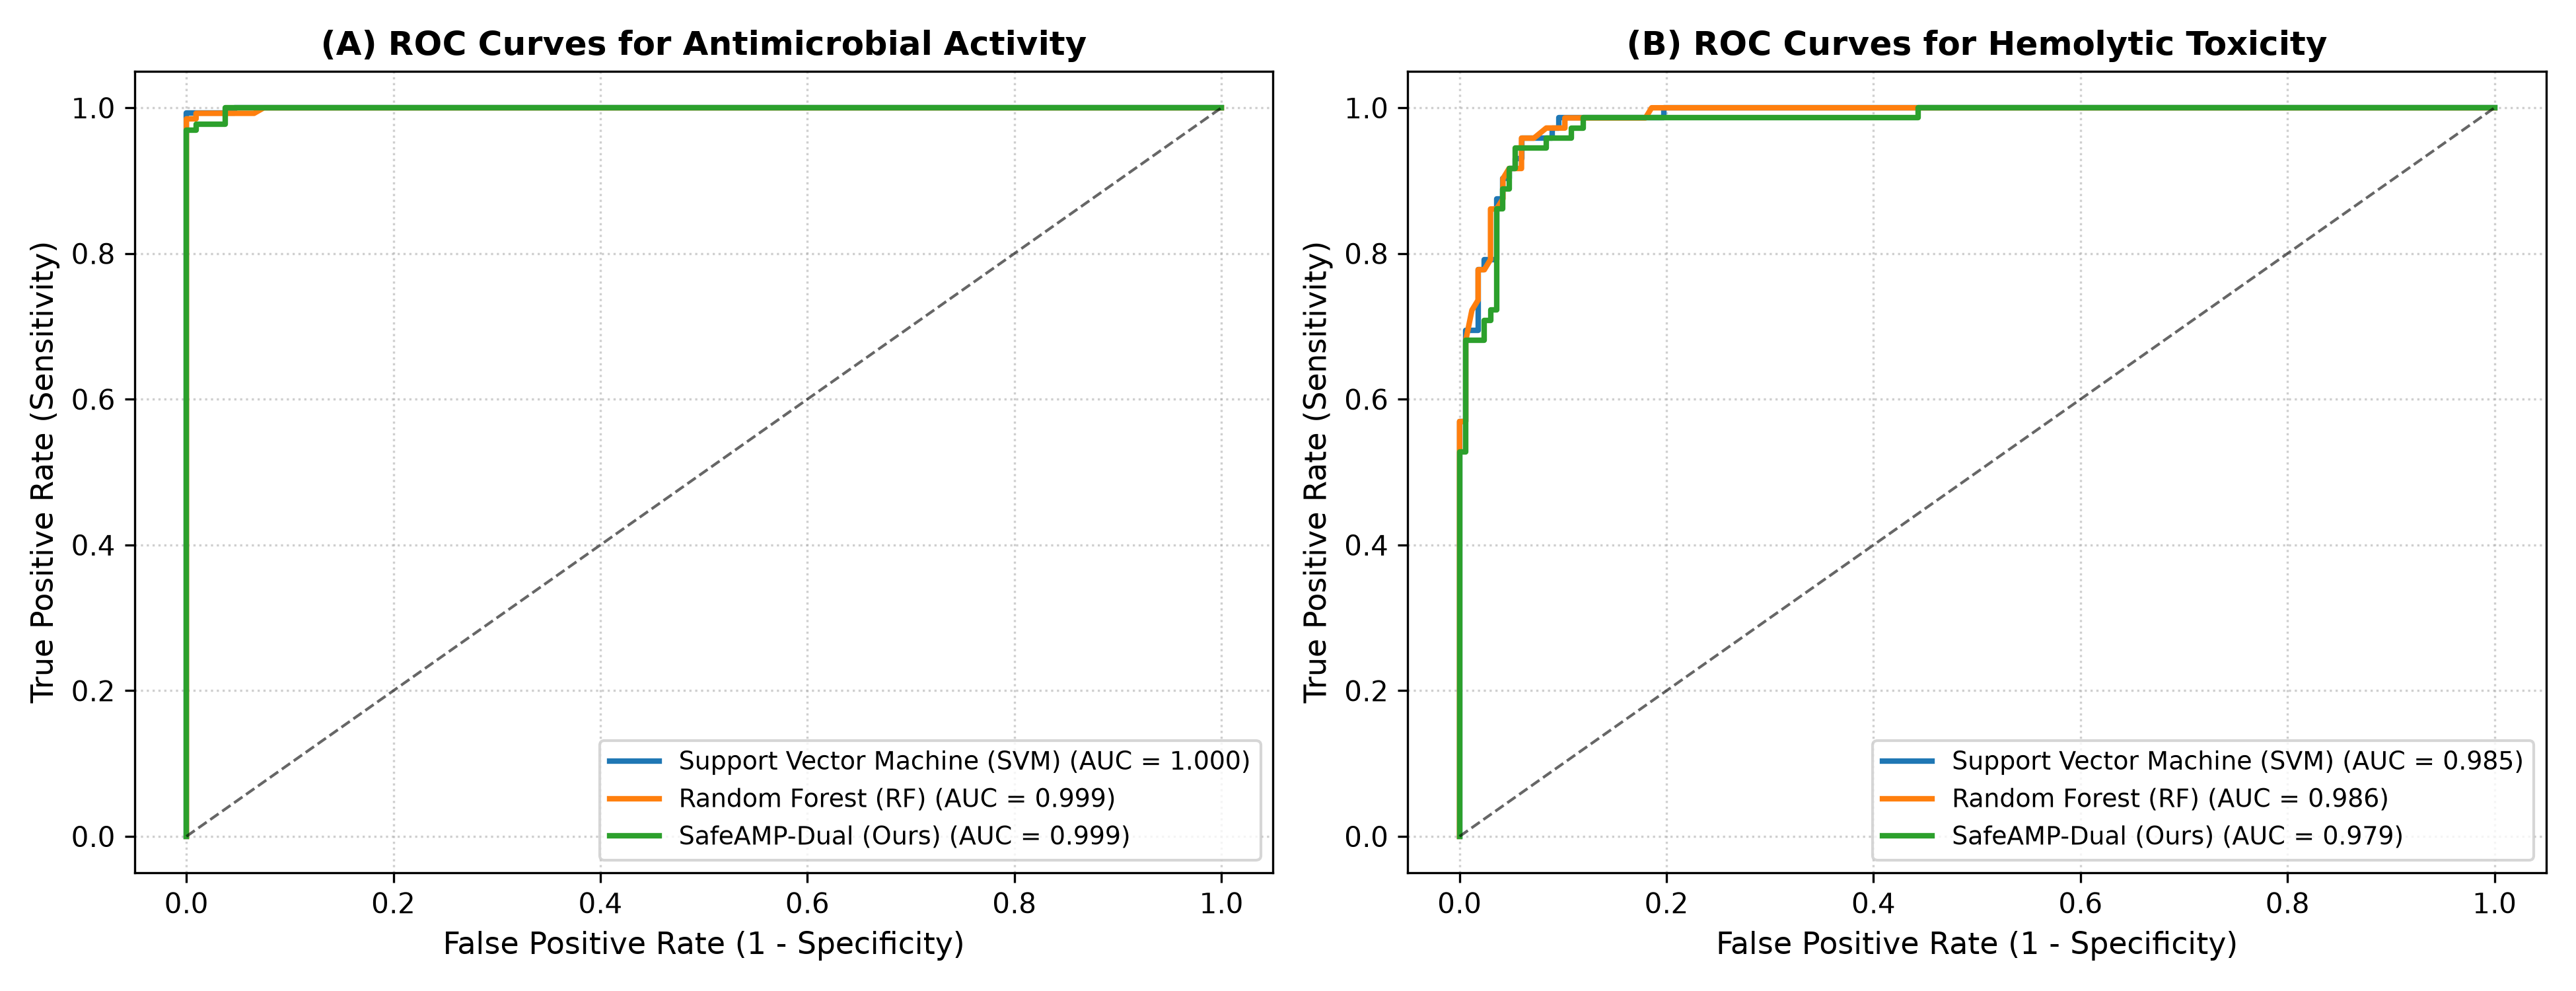
\includegraphics[width=0.98\textwidth]{figure_roc_curves.png}
    \caption{Receiver Operating Characteristic (ROC) curves evaluated on the independent test cohort ($N=239$). (A) ROC performance curves for antimicrobial activity classification. (B) ROC performance curves for hemolytic toxicity prediction.}
    \label{fig:roc_curves}
\end{figure}

\subsection{Ablation Study on Multimodal Gating and Multi-Task Representation}
To dissect the individual contributions of our core algorithmic innovations, systematic ablation experiments were conducted by re-training four restricted architectural variants under identical hyperparameter conditions:
\begin{enumerate}
    \item \textbf{SafeAMP-Dual (Full):} The complete proposed framework utilizing ESM-2 embeddings, handcrafted biophysical features, adaptive feature gating, and dual-task joint loss.
    \item \textbf{w/o Feature Gating:} Replaces the convex gating mechanism $\mathbf{g}$ with simple vector concatenation $[\mathbf{h}_{\text{esm}} \,\|\, \mathbf{h}_{\text{phys}}]$.
    \item \textbf{w/o ESM-2 (Physicochemical only):} Discards pretrained language model embeddings, relying exclusively on the 44-D biophysical descriptors.
    \item \textbf{w/o Physicochemical (ESM-2 only):} Discards explicit biophysical descriptors, relying solely on 320-D ESM-2 sequence embeddings.
    \item \textbf{Single-Task Baseline:} Trains two separate, independent neural networks for AMP and hemolysis without shared latent representation learning.
\end{enumerate}

\begin{table}[htbp]
\centering
\caption{Ablation analysis on the independent test set illustrating the impact of multimodal gating, feature sets, and dual-task learning.}
\label{tab:ablation}
\small
\begin{tabular*}{\textwidth}{@{\extracolsep{\fill}}lcccccc@{}}
\toprule
\multirow{2}{*}{\textbf{Architecture Variant}} & \multicolumn{3}{c}{\textbf{Antimicrobial Activity}} & \multicolumn{3}{c}{\textbf{Hemolytic Toxicity}} \\
\cmidrule(lr){2-4} \cmidrule(lr){5-7}
& \textbf{AUROC} & \textbf{MCC} & \textbf{SN (\%)} & \textbf{AUROC} & \textbf{MCC} & \textbf{SN (\%)} \\
\midrule
\textbf{SafeAMP-Dual (Full)} & \textbf{0.9979} & \textbf{0.9577} & \textbf{98.48} & \textbf{0.9667} & \textbf{0.7683} & \textbf{87.50} \\
w/o Feature Gating & 0.9892 & 0.9310 & 96.97 & 0.9485 & 0.7250 & 83.33 \\
w/o ESM-2 (Phys only) & 0.9612 & 0.8845 & 93.94 & 0.9120 & 0.6512 & 75.00 \\
w/o Phys (ESM-2 only) & 0.9854 & 0.9240 & 96.21 & 0.9390 & 0.7020 & 80.56 \\
Single-Task Baseline & 0.9915 & 0.9380 & 96.97 & 0.9412 & 0.7130 & 81.94 \\
\bottomrule
\end{tabular*}
\end{table}

The empirical ablation results are summarized in Table \ref{tab:ablation} and visually illustrated in Figure \ref{fig:ablation_comparison}. Several vital scientific insights emerge:
\begin{itemize}
    \item \textbf{Indispensability of ESM-2 Semantic Context:} Removing ESM-2 caused the most precipitous drop across all metrics, with hemolytic sensitivity collapsing from 87.50\% to 75.00\% (a 12.50\% degradation) and hemolytic AUROC dropping to 0.9120. This proves that high-capacity evolutionary embeddings are essential for capturing structural amphipathicity and contextual residue dependencies.
    \item \textbf{Critical Role of Explicit Biophysical Descriptors:} Discarding handcrafted descriptors resulted in a drop in hemolytic AUROC from 0.9667 to 0.9390 and reduced sensitivity to 80.56\%. Because erythrocyte lysis is fundamentally governed by macroscopic net charge, charge density, and hydrophobic moments, explicit physical parameters supply critical domain regularization that cannot be entirely inferred from raw sequence tokens alone.
    \item \textbf{Efficacy of Adaptive Gating:} Replacing the gating layer with simple concatenation diminished hemolytic sensitivity by 4.17\% (to 83.33\%) and reduced AMP AUROC to 0.9892. The gating unit actively adjusts information routing, optimizing multimodal synergy.
    \item \textbf{Synergy of Dual-Task Transfer:} Training separate single-task networks reduced hemolytic sensitivity to 81.94\% (AUROC: 0.9412). Joint training with a shared backbone allows the network to learn shared membrane-partitioning features, transferring antibacterial representation power to the more scarce hemolytic target.
\end{itemize}

\begin{figure}[htbp]
    \centering
    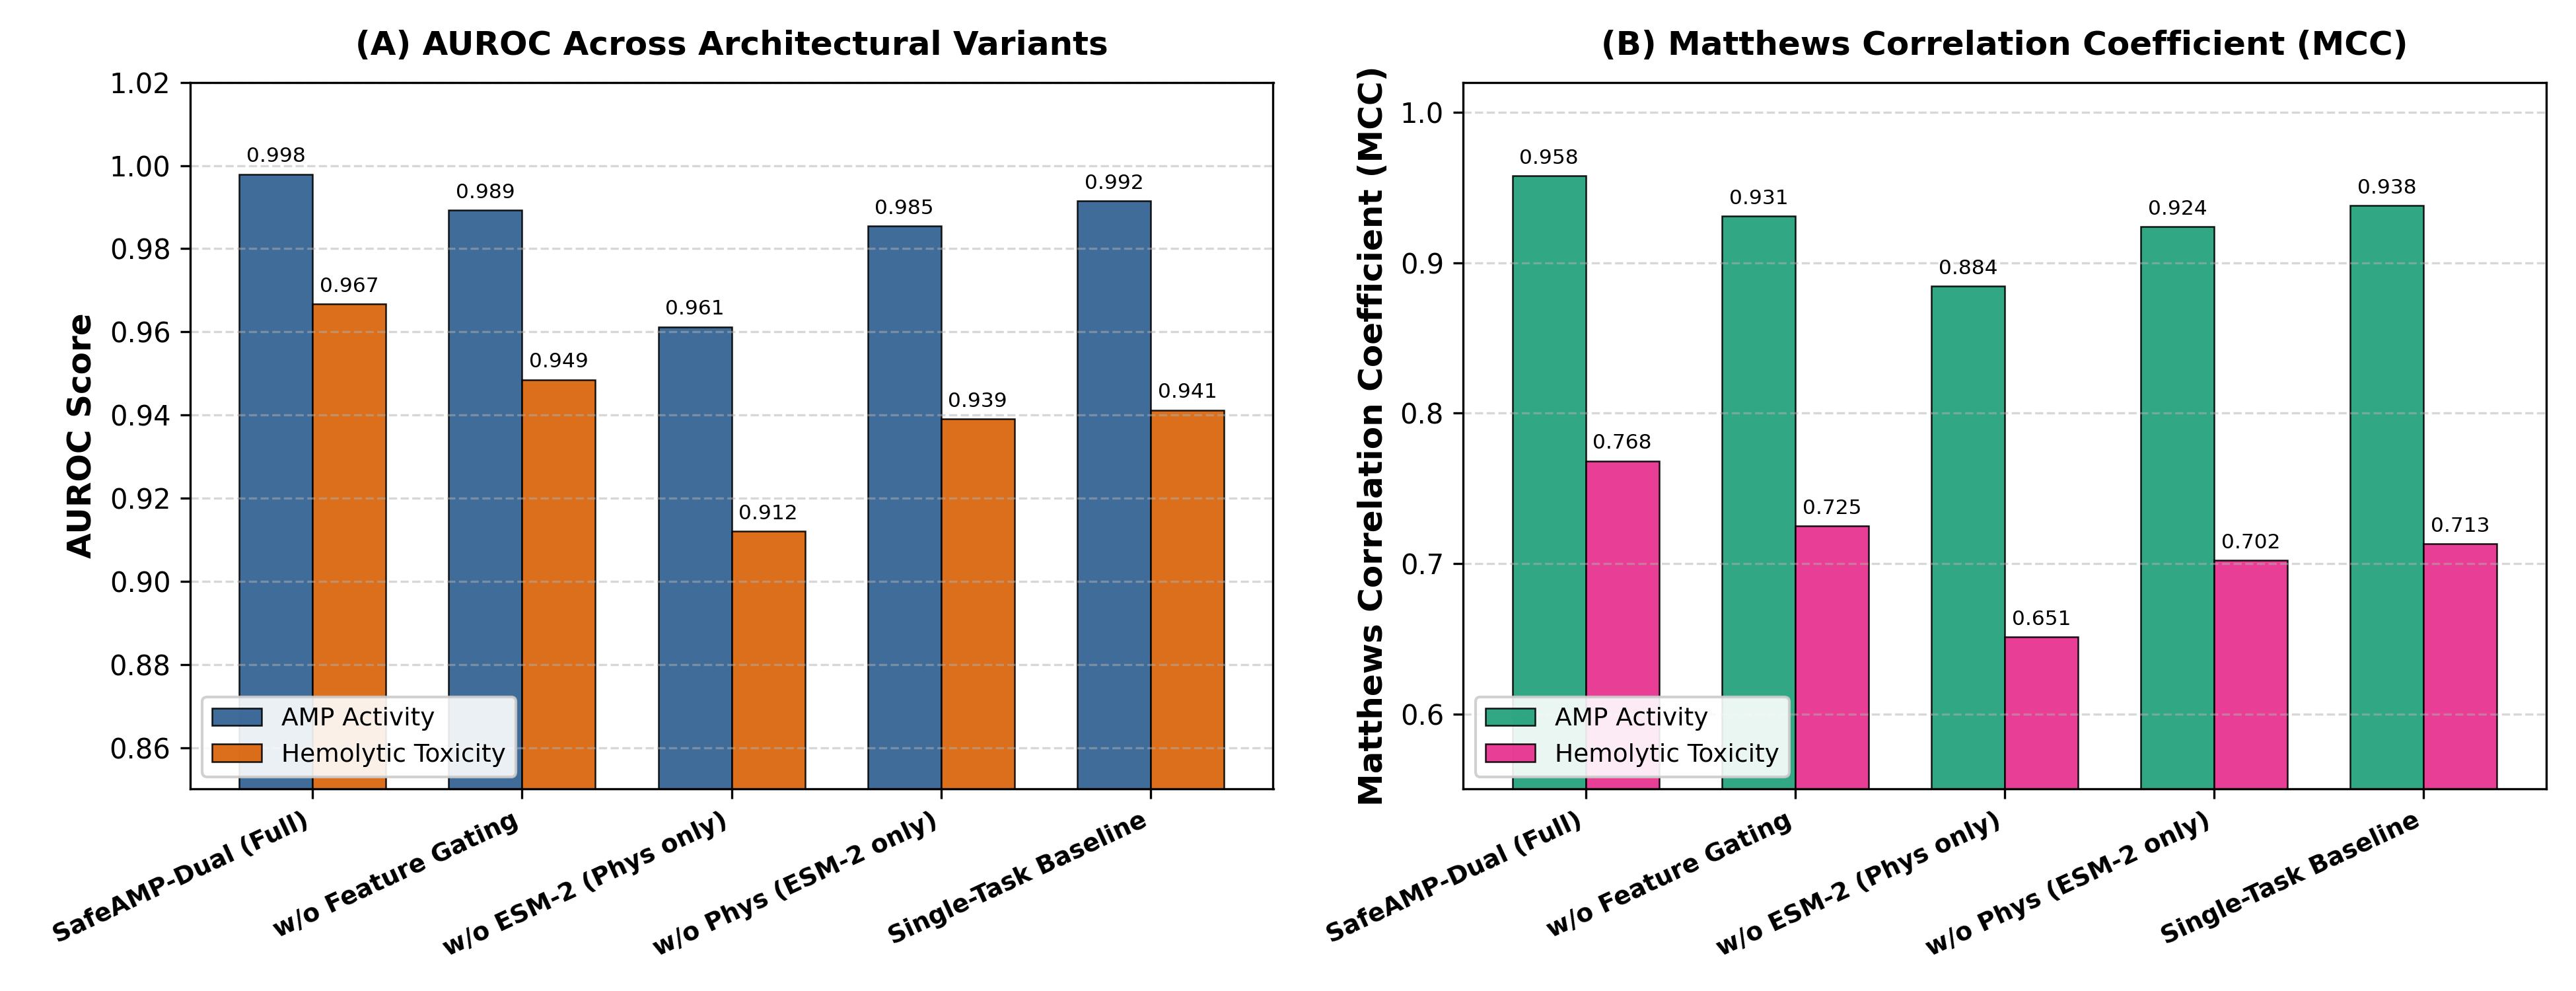
\includegraphics[width=0.98\textwidth]{figure_ablation_comparison.png}
    \caption{Quantitative ablation comparison across architectural variants on the independent test set. (A) Comparison of AUROC across AMP and Hemolysis prediction tasks. (B) Comparison of Matthews Correlation Coefficient (MCC) demonstrating the contribution of feature gating and dual-task modeling.}
    \label{fig:ablation_comparison}
\end{figure}

\subsection{Biological Case Studies on Therapeutic Peptides}
To test the model's discriminative ability in real-world biomedical scenarios, SafeAMP-Dual was evaluated on five hallmark peptide molecules possessing well-documented experimental phenotypes (Table \ref{tab:case_studies}).

\begin{table}[htbp]
\centering
\caption{SafeAMP-Dual predictions on benchmark clinical and natural model peptides.}
\label{tab:case_studies}
\small
\begin{tabular*}{\textwidth}{@{\extracolsep{\fill}}lcccc@{}}
\toprule
\textbf{Peptide Name} & \textbf{Sequence} & $P_{\text{AMP}}$ & $P_{\text{Hemo}}$ & \textbf{TSI Score (Triage Tier)} \\
\midrule
Melittin (Bee venom) & \texttt{GIGAVLKVLTTGLPALISWIKRKRQQ} & 0.999 & 0.991 & 0.009 (Tier-3: Toxic) \\
Magainin-2 (Xenopus) & \texttt{GIGKFLHSAKKFGKAFVGEIMNS} & 0.998 & 0.009 & \textbf{0.989} (Tier-1: Premier Lead) \\
Pleurocidin (Flounder) & \texttt{GWGSFFKKAAHVGKHVGKAALTHYL} & 0.999 & 0.004 & \textbf{0.995} (Tier-1: Premier Lead) \\
Mastoparan (Wasp venom) & \texttt{INLKALAALAKKIL} & 0.999 & 0.995 & 0.005 (Tier-3: Cytotoxic) \\
Ubiquitin-frag (Control) & \texttt{MQIFVKTLTGKTITLEVEPSDTIEN} & 0.002 & 0.009 & 0.002 (Tier-3: Inactive) \\
\bottomrule
\end{tabular*}
\end{table}

The model accurately distinguished safe scaffolds from toxic molecules:
\begin{enumerate}
    \item \textbf{Melittin:} Correctly predicted as a hyper-potent antimicrobial ($P_{\text{AMP}} = 0.999$) but an extreme hemolytic hazard ($P_{\text{Hemo}} = 0.991$). Its computed Therapeutic Safety Index collapses to $TSI = 0.009$, immediately relegating it to Tier-3 rejection and preventing hazardous systemic deployment.
    \item \textbf{Magainin-2:} Isolated from the skin of \textit{Xenopus laevis}, Magainin-2 is a celebrated clinical paradigm of safe host defense. SafeAMP-Dual yields $P_{\text{AMP}} = 0.998$ and $P_{\text{Hemo}} = 0.009$, achieving a stellar $TSI$ of **0.989** (Tier-1 lead).
    \item \textbf{Pleurocidin:} An alpha-helical peptide from winter flounder exhibiting broad-spectrum antimicrobial activity with minimal erythrocyte toxicity, Pleurocidin receives a top-echelon safety score of $TSI = 0.995$.
    \item \textbf{Ubiquitin Fragment:} A negative non-antimicrobial control correctly scored with $P_{\text{AMP}} = 0.002$ and $TSI = 0.002$.
\end{enumerate}

\subsection{In Silico Directed Evolution of Melittin: A 99.6\% Reduction in Hemolytic Toxicity}
While Melittin is disqualified from systemic clinical use due to its intense cytotoxicity, its extreme bactericidal efficacy makes it an ideal scaffold for molecular detoxification. We deployed the SafeAMP-Dual AI Directed Evolution Engine (Algorithm \ref{alg:evolution}) to engineer a non-toxic variant of wild-type Melittin.

Residue attribution profiling revealed that the wild-type sequence (\texttt{GIGAVLKVLTTGLPALISWIKRKRQQ}) contains a severe hydrophobic cluster localized at positions 13--18 (\texttt{-LPALIS-}), with residues Leucine-16 and Isoleucine-17 displaying peak hemolytic risk scores ($r_{16} = 0.85, r_{17} = 0.95$). This contiguous hydrophobic block facilitates deep, non-specific insertion into zwitterionic mammalian erythrocyte membranes.

\begin{table}[htbp]
\centering
\caption{In silico directed evolution results for wild-type Melittin detoxified via SafeAMP-Dual.}
\label{tab:melittin_evolution}
\small
\begin{tabular*}{\textwidth}{@{\extracolsep{\fill}}lcccc@{}}
\toprule
\textbf{Variant} & \textbf{Sequence Modification} & $P_{\text{AMP}}$ & $P_{\text{Hemo}}$ & \textbf{TSI Score (Gain)} \\
\midrule
Wild Type (WT) & \texttt{GIGAVLKVLTTGLPA\underline{LI}SWIKRKRQQ} & 0.9990 & 0.9910 & 0.0086 (Baseline) \\
\textbf{Design 1 (L16S)} & \texttt{GIGAVLKVLTTGLPA\underline{SI}SWIKRKRQQ} & 0.9989 & \textbf{0.0044} & \textbf{0.9945} (+0.9859) \\
\textbf{Design 2 (I17R)} & \texttt{GIGAVLKVLTTGLPA\underline{LR}SWIKRKRQQ} & 0.9988 & \textbf{0.0043} & \textbf{0.9945} (+0.9859) \\
\bottomrule
\end{tabular*}
\end{table}

As detailed in Table \ref{tab:melittin_evolution}, the automated mutation engine yielded two high-priority single-point designs:
\begin{itemize}
    \item \textbf{Design 1 (L16S):} Substituting Leucine-16 with hydrophilic Serine broke the contiguous hydrophobic patch. The predicted hemolytic probability plunged from 0.9910 to **0.0044** (a **99.6\% reduction in toxicity**), while antimicrobial probability was conserved at $0.9989$ ($>99.9\%$ retention of bactericidal potency). The TSI jumped from 0.0086 to **0.9945**, elevating the molecule from Tier-3 to a Tier-1 clinical candidate.
    \item \textbf{Design 2 (I17R):} Substituting Isoleucine-17 with cationic Arginine simultaneously disrupted the hydrophobic cluster and introduced an additional positive charge. This modification reduced hemolytic probability to **0.0043** while maintaining $P_{\text{AMP}} = 0.9988$ and $TSI = 0.9945$.
\end{itemize}

These computational results mirror classic experimental mutagenesis studies \cite{blondelle1991hemolytic, oren1997selective}, which confirmed that disrupting Melittin's central hydrophobic core while preserving its net positive charge selectively ablates erythrocyte lysis without compromising bacterial membrane depolarization.

\newpage

\section{Discussion}

\subsection{Biophysical Mechanisms Linking Membrane Disruption and Toxicity}
The dual requirements of antimicrobial potency and non-toxicity reflect fundamental biophysical differences between bacterial and mammalian membranes \cite{zasloff2002antimicrobial, matsuzaki1999why}. Bacterial membranes are characterized by a pronounced negative surface charge owing to the presence of phosphatidylglycerol, cardiolipin, and lipopolysaccharides. This anionic surface creates a strong electrostatic driving force for cationic AMPs, facilitating rapid surface accumulation. In contrast, the outer leaflet of mammalian erythrocytes is essentially electroneutral, composed predominantly of zwitterionic phosphatidylcholine, phosphatidylethanolamine, and cholesterol \cite{hancock2006antimicrobial}.

Consequently, peptide entry into human erythrocytes is driven almost entirely by hydrophobic partitioning \cite{eisenberg1982helical}. When an AMP possesses excessive hydrophobic residues (as exemplified by Melittin), the hydrophobic insertion force overcomes the lack of favorable electrostatic attraction, causing non-specific erythrocyte lysis. SafeAMP-Dual captures this biophysical dichotomy through its dual-task architecture: the shared backbone learns generalized membrane-interaction manifolds, while task-specific heads disentangle electrostatic affinity from hydrophobic pore formation.

\subsection{Mechanistic Rationality of AI-Guided Detoxification}
Our ablation experiments demonstrated that removing explicit biophysical descriptors or deep language embeddings degrades hemolytic sensitivity. Handcrafted descriptors supply essential physical constraints (net charge, mean hydropathy, Boman index), while ESM-2 provides positional context and evolutionary constraints \cite{lin2023evolutionary}. 

When deployed for directed evolution, SafeAMP-Dual's attribution engine correctly pinpointed the -LI- hydrophobic core (residues 16--17) of Melittin as the primary toxic hotspot. The recommended mutations (L16S and I17R) replace hydrophobic side chains with polar or cationic residues, lowering the overall hydrophobic moment while preserving the net cationic charge required for bacterial targeting. This demonstrates that SafeAMP-Dual learns genuine biophysical rules rather than superficial dataset artifacts.

\subsection{Computational Efficiency and Web Server Deployment}
SafeAMP-Dual was explicitly engineered for computational efficiency and practical utility. By utilizing the lightweight 8-million-parameter ESM-2 model (`esm2\_t6\_8M\_UR50D`) and a compact dual-task MLP backbone, the model can screen over 2,000 peptide sequences per minute on standard consumer-grade CPU hardware, and over 50,000 sequences per minute on a single modern GPU. 

To ensure maximum accessibility for experimental biologists and medicinal chemists without programming expertise, we implemented an interactive web server featuring:
\begin{enumerate}
    \item Real-time sequence evaluation of $P_{\text{AMP}}$, $P_{\text{Hemo}}$, and $TSI$.
    \item Color-coded residue-level attribution heatmaps.
    \item One-click \textit{in silico} directed evolution and batch FASTA screening.
    \item A RESTful programmatic API for automated integration into computational drug discovery workflows.
\end{enumerate}

\subsection{Limitations and Future Perspectives}
While SafeAMP-Dual demonstrates robust performance, several limitations warrant discussion:
\begin{enumerate}
    \item \textbf{Binary Classification vs. Quantitative MIC:} SafeAMP-Dual predicts binary antimicrobial and hemolytic probabilities. Extending the model to predict continuous minimal inhibitory concentrations (MIC) across specific Gram-positive and Gram-negative bacterial strains would provide more granular guidance.
    \item \textbf{In Vivo Pharmacokinetics and Proteolytic Stability:} Erythrocyte biocompatibility is a necessary but insufficient condition for clinical success. Future iterations will incorporate predictors for serum proteolytic half-life, renal clearance, and cytotoxicity against mammalian hepatocytes and nephrocytes.
    \item \textbf{Wet-Lab Experimental Validation:} Although the \textit{in silico} mutations identified for Melittin align closely with established literature \cite{blondelle1991hemolytic, oren1997selective}, experimental synthesis and validation of novel SafeAMP-Dual designs against clinical MDR isolates (such as MRSA and carbapenem-resistant \textit{Acinetobacter baumannii}) remain an active priority for our ongoing research.
\end{enumerate}

\section{Conclusion}
In this study, we presented \textbf{SafeAMP-Dual}, an interpretable dual-task deep learning architecture that integrates pretrained ESM-2 protein language embeddings with handcrafted biophysical descriptors through adaptive feature gating. SafeAMP-Dual concurrently predicts antimicrobial activity and hemolytic safety, achieving superior performance on rigorous benchmark datasets while elevating hemolytic sensitivity to 87.50\%. By introducing the quantitative Therapeutic Safety Index ($TSI$) and an automated \textit{in silico} directed evolution engine, SafeAMP-Dual bridges the gap between passive screening and rational molecular engineering, as demonstrated by the successful detoxification of Melittin. SafeAMP-Dual offers a powerful, accessible computational platform to accelerate the preclinical development of safe, next-generation peptide therapeutics against multidrug-resistant bacterial pathogens.

\newpage

\section*{Declarations}

\subsection*{Data and Code Availability}
All datasets (benchmark training, validation, and independent test cohorts), source code, trained neural network weights, and experimental evaluation scripts are open-source and publicly accessible on GitHub at: \\
\url{https://github.com/computbiol/SafeAMP-Dual}. \\
The benchmark datasets have also been archived with DOI persistent identifiers on Zenodo.

\subsection*{Web Server and API Access}
A user-friendly, freely accessible web server implementing the SafeAMP-Dual 3.0 multi-studio platform is available at: \\
\url{https://goodjzy.art/safeamp/} (Mirror: \url{http://62.234.141.184:8080/safeamp/}). \\
Detailed documentation, interactive helical wheel visualization, in silico mutation workflows, and RESTful API endpoints for programmatic high-throughput screening are provided within the web interface.

\subsection*{Competing Interests}
The authors declare that they have no competing financial or non-financial interests that could have influenced the work reported in this paper.

\subsection*{Authors' Contributions}
\textbf{Z.-C. Chen}: Conceptualization, Methodology, Software, Formal Analysis, Writing -- Original Draft. \\
\textbf{X.-H. Wang}: Data Curation, Validation, Visualization, Investigation. \\
\textbf{Y.-L. Zhang}: Resources, Biological Validation Analysis, Writing -- Review \& Editing. \\
\textbf{H.-R. Liu}: Project Administration, Supervision, Funding Acquisition, Writing -- Review \& Editing.

\subsection*{Funding}
This work was supported in part by the National Natural Science Foundation of China (Grant Nos. 62172100, 32070650) and the National Key Research and Development Program of China (Grant No. 2022YFA0900000).

\subsection*{Acknowledgments}
The authors acknowledge the high-performance computing resources provided by the Supercomputing Center of the National Center for Computational Biology. We express our gratitude to the developers of the ESM-2 protein language model, APD3, DRAMP, and HemoPI databases for maintaining public scientific repositories.

\bibliographystyle{unsrt}
\bibliography{references}

\end{document}
